\chapter{Analisi e Progettazione delle Espansioni}

L'esperienza maturata durante l'esercitazione Locked Shields 2025 ha fornito insight fondamentali per guidare l'evoluzione di VolWeb. L'utilizzo della piattaforma in un contesto operativo ad alta pressione ha evidenziato sia i punti di forza che le limitazioni dell'implementazione originale, fornendo una roadmap chiara per le espansioni necessarie.

Durante Locked Shields, la necessità di analizzare rapidamente dump di memoria per identificare indicatori di compromissione ha reso evidente l'assenza di capacità di pattern matching avanzato. Gli analisti erano costretti a fare affidamento esclusivamente sui plugin predefiniti di Volatility, limitando significativamente la capacità di identificare minacce custom o varianti di malware conosciuti. Questa limitazione operativa ha motivato l'integrazione di YARA come priorità principale per le espansioni di VolWeb.

\section{Analisi dei Requisiti}

\subsection{Studio delle limitazioni di VolWeb originale}

L'analisi delle limitazioni di VolWeb è stata condotta attraverso tre prospettive complementari: l'esperienza diretta durante Locked Shields 2025, l'analisi del codice sorgente della versione originale, e il feedback raccolto dalla community degli utilizzatori.

Durante l'esercitazione Locked Shield, diverse limitazioni sono emerse con particolare evidenza. La più critica riguardava l'assenza di supporto per YARA, che impediva l'implementazione di capacità di threat hunting proattive. In uno scenario dove i red team utilizzavano malware custom e tecniche di evasione sofisticate, la capacità di definire e applicare pattern di ricerca specifici sarebbe stata fondamentale per l'identificazione rapida delle compromissioni.

L'architettura di autenticazione originale, basata su JWT e sessioni utente persistenti, si è rivelata un overhead non necessario nel contesto di deployment isolati tipici degli ambienti di analisi forense. Durante Locked Shields, dove ogni blue team operava in un ambiente segregato, la gestione degli utenti e delle sessioni aggiungeva complessità senza fornire valore reale. Questa osservazione ha portato alla decisione di semplificare l'architettura rimuovendo il layer di autenticazione nelle espansioni.

Similmente, il supporto per cloud storage (S3) presente nella versione originale si è dimostrato non necessario e potenzialmente problematico dal punto di vista della sicurezza. In ambienti forensi, dove i dump di memoria contengono dati estremamente sensibili, l'upload su storage cloud introduce rischi di data exfiltration e compliance. Durante Locked Shield, tutti i team hanno utilizzato esclusivamente storage locale, confermando che il supporto cloud non era una priorità per il target audience di VolWeb.

Un aspetto critico emerso durante l'esercitazione riguarda la resilienza dell'infrastruttura in scenari di cyber warfare simulato. Durante Locked Shields, i servizi cloud erano tra i primi target degli attacchi del red team, rendendo potenzialmente inaccessibili le evidenze archiviate remotamente proprio nel momento di maggior necessità. Questa esperienza ha confermato che affidarsi a storage cloud per evidenze forensi critiche introduce un single point of failure inaccettabile. In uno scenario reale di incident response, dove l'infrastruttura aziendale potrebbe essere compromessa o i servizi cloud potrebbero essere target di DDoS o altri attacchi, la disponibilità locale delle evidenze diventa essenziale per garantire la continuità delle operazioni di analisi forense.

\subsection{Identificazione delle aree di miglioramento}

Basandosi sull'analisi delle limitazioni e sull'esperienza operativa, sono state identificate due aree principali di miglioramento che guidano lo sviluppo delle espansioni.

La prima e più critica area riguarda l'integrazione di YARA per fornire capacità di pattern matching e threat hunting. Questa integrazione deve permettere agli analisti di caricare e gestire rule files, organizzarli in rulesets logici, eseguire scansioni e visualizzare i risultati con contesto forense appropriato. Il sistema deve inoltre supportare la validazione automatica delle regole al momento del caricamento, garantendo che solo regole sintatticamente corrette vengano applicate durante le analisi.

La seconda area si concentra sulla semplificazione dell'architettura rimuovendo componenti non essenziali. L'eliminazione del sistema di autenticazione e del supporto cloud storage riduce la complessità del deployment e manutenzione, permettendo agli analisti di concentrarsi sulle funzionalità core di analisi forense. Questa semplificazione garantisce inoltre maggiore resilienza operativa, eliminando dipendenze esterne che potrebbero diventare non disponibili proprio durante incidenti critici.

\subsection{Requisiti funzionali e non funzionali}

I requisiti per le espansioni di VolWeb sono stati definiti con un focus specifico sull'integrazione YARA e sulle semplificazioni architetturali identificate.

\begin{tabularx}{\textwidth}{|c|X|c|c|}
\caption{Requisiti Funzionali del Sistema}
\label{tab:requisiti-funzionali} \\
\hline
\textbf{ID} & \textbf{Descrizione} & \textbf{Priorità} & \textbf{Area} \\
\hline
RF01 & Upload di file di regole YARA da file system (.yar) & Alta & YARA \\
\hline
RF02 & Import di regole YARA da repository github & Alta & YARA \\
\hline
RF03 & Creazione manuale o editing di regole YARA tramite editor integrato & Alta & YARA \\
\hline
RF04 & Validazione sintattica delle regole YARA al momento dell'upload & Alta & YARA \\
\hline
RF05 & Visualizzazione delle regole caricate con syntax highlighting & Media & YARA \\
\hline
RF06 & Eliminazione di regole YARA non più necessarie & Media & YARA \\
\hline
RF07 & Organizzazione delle regole in rulesets logici & Alta & YARA \\
\hline
RF08 & Creazione e gestione di rulesets personalizzati & Alta & YARA \\
\hline
RF09 & Esecuzione di scansioni YARA su dump completi & Alta & YARA \\
\hline
RF10 & Selezione di regole specifiche o rulesets per la scansione & Alta & YARA \\
\hline
RF11 & Visualizzazione dei match YARA con contesto (offset, processo) & Alta & YARA \\
\hline
RF13 & Rimozione del sistema di autenticazione utente & Alta & Architettura \\
\hline
RF14 & Rimozione del supporto per cloud storage (S3) & Alta & Architettura \\
\hline
RF15 & Accesso diretto all'applicazione senza login & Alta & Architettura \\
\hline
RF16 & Semplificazione del modello dati rimuovendo user associations & Media & Architettura \\
\hline
\end{tabularx}

\begin{tabularx}{\textwidth}{|c|X|c|c|}
\caption{Requisiti Non Funzionali del Sistema} \label{tab:requisiti-non-funzionali} \\
\hline
\textbf{ID} & \textbf{Descrizione} & \textbf{Priorità} & \textbf{Categoria} \\
\hline
RNF01 & UI responsive durante scansioni YARA & Alta & Usabilità \\
\hline
RNF02 & Compatibilità con YARA 4.x syntax & Alta & Compatibilità \\
\hline
RNF03 & Storage su Postgresql dei file di regole e risultati & Alta & Sicurezza \\
\hline
RNF04 & Nessuna dipendenza da servizi cloud esterni & Alta & Sicurezza \\
\hline
RNF05 & Deployment semplificato senza configurazione auth & Alta & Deployment \\
\hline
RNF06 & Gestione efficiente di rulesets con centinaia di regole & Alta & Performance \\
\hline
\end{tabularx}

\subsection{Requisiti specifici per la gestione YARA}

L'integrazione di YARA in VolWeb richiede particolare attenzione ai dettagli implementativi per garantire un'esperienza utente fluida e funzionalità forensi efficaci.

\subsubsection{Gestione delle regole}

Il sistema deve permettere l'upload di file di regole YARA attraverso un'interfaccia intuitiva. I file supportati devono includere l'estensione standard .yar e il sistema deve gestire sia l'upload di file singoli, sia l'import di regole multiple direttamente da repository github pubbliche, che la creazione contestuale di regole YARA su file editor integrato. Al momento dell'upload, ogni file deve essere validato utilizzando il parser YARA per garantire una sintassi corretta prima del salvataggio.

Le regole caricate devono essere persistite nel database Postgresql. Questa scelta di storage garantisce che le regole rimangano sempre accessibili, indipendentemente dallo stato della rete o di servizi esterni. Ogni regola deve mantenere metadati quali nome del file originale, data di upload, e hash per verifica di integrità. Il sistema deve fornire una vista delle regole caricate con syntax highlighting appropriato per il linguaggio YARA, facilitando la review e comprensione delle regole.

\subsubsection{Organizzazione in rulesets}

Un aspetto fondamentale per l'usabilità del sistema è la capacità di organizzare le regole YARA in rulesets logici. Gli analisti forensi spesso lavorano con centinaia di regole diverse, e la capacità di raggrupparle per categoria, famiglia di malware, o tipo di analisi diventa essenziale per un workflow efficiente.

Il sistema deve permettere la creazione di rulesets personalizzati dove gli utenti possono raggruppare regole correlate. Ogni ruleset deve avere un nome descrittivo e una descrizione opzionale.

L'interfaccia deve fornire funzionalità di gestione dei rulesets inclusa la creazione di nuovi rulesets, l'aggiunta o rimozione di regole da un ruleset, la visualizzazione delle regole contenute in un ruleset, e l'eliminazione di rulesets non più necessari. Durante la selezione delle regole per una scansione, gli utenti devono poter selezionare interi rulesets oltre a regole individuali, semplificando significativamente il processo per analisi che richiedono l'applicazione di molte regole.

\subsubsection{Esecuzione delle scansioni}

L'esecuzione delle scansioni YARA deve essere integrata nel workflow esistente di VolWeb. Quando un utente seleziona un dump per l'analisi, deve essere presentata l'opzione di eseguire scansioni YARA utilizzando le regole caricate. Il sistema deve permettere la selezione granulare di quali regole applicare, con opzioni per selezionare tutte le regole, rulesets specifici, o combinazioni personalizzate di regole individuali.

Durante l'esecuzione, il sistema deve fornire feedback sul progresso e includere il numero di match trovati. Le scansioni devono essere eseguite in modo asincrono attraverso Celery per non bloccare l'interfaccia utente, con la possibilità di continuare altre attività mentre la scansione procede. Il sistema deve ottimizzare l'esecuzione quando vengono selezionati rulesets completi, compilando tutte le regole del set in un'unica operazione per migliorare le performance.

\subsubsection{Presentazione dei risultati}

I risultati delle scansioni YARA devono essere presentati in modo che faciliti l'analisi forense. Ogni match deve includere il nome della regola che ha generato il match, il ruleset di appartenenza se applicabile, l'offset esatto nel dump dove il pattern è stato trovato, il contesto del processo se applicabile, e un hex dump della regione di memoria circostante.

La visualizzazione deve permettere il filtering e il sorting dei risultati per facilitare l'analisi di grandi numeri di match. Gli utenti devono poter filtrare i risultati per ruleset, permettendo di focalizzarsi su specifiche categorie di minacce. Il sistema deve implementare una deduplicazione intelligente per evitare di mostrare match ripetitivi che non aggiungono valore all'analisi, con particolare attenzione quando multiple regole dello stesso ruleset identificano lo stesso artefatto.

\section{Implementazione delle Espansioni YARA}

L'implementazione delle funzionalità YARA in VolWeb ha richiesto un'attenta progettazione architetturale per garantire integrazione fluida con l'infrastruttura esistente, mantenendo al contempo elevate performance e usabilità. L'approccio modulare adottato ha permesso di estendere la piattaforma senza disruption delle funzionalità core.

\subsection{Architettura Backend del Modulo YARA}

L'integrazione YARA è stata realizzata attraverso due nuovi moduli Django: \texttt{yararules} e \texttt{yararulesets}, che gestiscono rispettivamente le regole individuali e i loro raggruppamenti logici. Questa separazione permette massima flessibilità nell'organizzazione delle regole, facilitando sia operazioni su singole regole che su collezioni complesse.

\subsubsection{Modello e Gestione delle Regole}

Il modello \texttt{YaraRule} implementa una struttura dati completa per la gestione delle regole YARA:

\begin{minted}[
    breaklines,
    frame=lines,
    framesep=2mm,
    baselinestretch=1.2,
    fontsize=\small,
    linenos
]{python}
class YaraRule(models.Model):
    """
    YaraRule Model
    Holds the important metadata about the YARA rule.
    """

    id = models.AutoField(primary_key=True)
    name = models.CharField(max_length=250)
    etag = models.CharField(max_length=256, unique=True)
    rule_content = models.TextField()
    description = models.TextField(null=True, blank=True)
    linked_yararuleset = models.ForeignKey(YaraRuleSet, on_delete=models.CASCADE, null=True)
    status = models.IntegerField(default=0)
    url = models.TextField(null=True)
    source = models.CharField(max_length=10, choices=RULE_SOURCES, null=True)
    is_active = models.BooleanField(default=True)
\end{minted}

Il campo \texttt{status} implementa un sistema di stati per tracciare la validazione delle regole (0: pending, -1: empty content error, -2: syntax error, -3: general error code, -4: unknown error, 100: valid), mentre \texttt{source} distingue tra regole create manualmente o importate da repository GitHub. L'utilizzo di un \texttt{etag} univoco, calcolato come hash del contenuto, previene duplicazioni accidentali e facilita la sincronizzazione.

\subsubsection{Serializer e Validazione delle Regole}

Il \texttt{YaraRuleSerializer} è un serializer che si occupa non solo della serializzazione dei modelli \texttt{YaraRule}, ma anche della gestione sicura delle relazioni e dell'attivazione automatica dei task asincroni di validazione.

Il campo \texttt{ruleset\_name}, calcolato tramite il serializer, espone in sola lettura il nome del \texttt{YaraRuleSet} collegato. Il metodo \texttt{to\_representation} è stato sovrascritto per includere in modo robusto i dettagli del \texttt{linked\_yararuleset}, evitando errori in caso di cancellazioni a cascata.

In fase di creazione (\texttt{create}), il serializer salva la regola e avvia immediatamente la validazione asincrona della stessa tramite il task \texttt{start\_yararule\_validation}. Se la regola è associata a un RuleSet, viene aggiornato anche lo stato di quest’ultimo e viene triggerata la validazione del set con \texttt{start\_ruleset\_validation}.

Durante l’aggiornamento (\texttt{update}), il serializer rileva se sono cambiate parti sensibili come il contenuto della regola o l’associazione al RuleSet. In tal caso, oltre a far ripartire la validazione della regola stessa, provvede a riavviare anche la validazione del RuleSet precedente (se la regola è stata spostata) e di quello corrente, garantendo così la coerenza dello stato di validazione complessivo.:

\begin{minted}[
    breaklines,
    frame=lines,
    framesep=2mm,
    baselinestretch=1.2,
    fontsize=\small,
    linenos
]{python}
class YaraRuleSerializer(serializers.ModelSerializer):
    ruleset_name = serializers.CharField(source='linked_yararuleset.name', read_only=True, allow_null=True)
    
    class Meta:
        model = YaraRule
        fields = "__all__"
    
    def to_representation(self, instance):
        """
        Override to add linked_yararuleset information safely
        """
        data = super().to_representation(instance)
        
        # Handle the case where linked_yararuleset might not exist anymore (e.g., during cascade delete)
        try:
            if hasattr(instance, 'linked_yararuleset') and instance.linked_yararuleset:
                data['linked_yararuleset'] = {
                    'id': instance.linked_yararuleset.id,
                    'name': instance.linked_yararuleset.name
                }
            else:
                data['linked_yararuleset'] = None
        except YaraRuleSet.DoesNotExist:
            # This can happen during cascade deletes when the ruleset is deleted first
            data['linked_yararuleset'] = None
        
        return data
    
    def create(self, validated_data):
        """
        Create a new YARA rule.
        """
        # Create the rule instance
        rule = super().create(validated_data)
        
        # Trigger validation
        try:
            from volatility_engine.tasks import start_yararule_validation
            start_yararule_validation.delay(rule.id)
        except ImportError:
            logger.warning("Could not import start_yararule_validation task")
        except Exception as e:
            logger.error(f"Error triggering rule validation: {e}")
        
        # Trigger ruleset validation if linked
        if rule.linked_yararuleset:
            try:
                rule.linked_yararuleset.status = 0
                rule.linked_yararuleset.save()
                
                from volatility_engine.tasks import start_ruleset_validation
                start_ruleset_validation.delay(rule.linked_yararuleset.id)
            except ImportError:
                logger.warning("Could not import start_ruleset_validation task")
            except Exception as e:
                logger.error(f"Error triggering ruleset validation: {e}")
        
        return rule
    
    def update(self, instance, validated_data):
        """
        Update a YARA rule.
        """
        # Store old content for comparison
        old_content = instance.rule_content
        old_ruleset = instance.linked_yararuleset
        
        # Update the instance
        rule = super().update(instance, validated_data)
        
        # Check if content changed
        content_changed = 'rule_content' in validated_data and old_content != rule.rule_content
        
        # Check if ruleset changed
        ruleset_changed = 'linked_yararuleset' in validated_data and old_ruleset != rule.linked_yararuleset
        
        # Trigger revalidation if content changed
        if content_changed:
            rule.status = 0
            rule.save(update_fields=['status'])
            
            try:
                from volatility_engine.tasks import start_yararule_validation
                start_yararule_validation.delay(rule.id)
            except ImportError:
                logger.warning("Could not import start_yararule_validation task")
            except Exception as e:
                logger.error(f"Error triggering rule validation: {e}")
        
        # Trigger ruleset revalidation if needed
        if content_changed or ruleset_changed:
            # Revalidate old ruleset if rule was removed from it
            if ruleset_changed and old_ruleset:
                try:
                    old_ruleset.status = 0
                    old_ruleset.save()
                    
                    from volatility_engine.tasks import start_ruleset_validation
                    start_ruleset_validation.delay(old_ruleset.id)
                except ImportError:
                    logger.warning("Could not import start_ruleset_validation task")
                except Exception as e:
                    logger.error(f"Error triggering old ruleset validation: {e}")
            
            # Revalidate new/current ruleset
            if rule.linked_yararuleset:
                try:
                    rule.linked_yararuleset.status = 0
                    rule.linked_yararuleset.save()
                    
                    from volatility_engine.tasks import start_ruleset_validation
                    start_ruleset_validation.delay(rule.linked_yararuleset.id)
                except ImportError:
                    logger.warning("Could not import start_ruleset_validation task")
                except Exception as e:
                    logger.error(f"Error triggering ruleset validation: {e}")
        
        return rule
\end{minted}

\subsubsection{Modello e gestione dei RuleSets}
Il modello \texttt{YaraRuleSet} rappresenta un insieme logico di regole YARA, permettendo di raggrupparle in collezioni coerenti. Oltre ai campi base come \texttt{name} e \texttt{description}, include un campo \texttt{compiled\_rules} per memorizzare direttamente la versione compilata delle regole, utile per ottimizzare l'esecuzione dei controlli. Il campo \texttt{is\_default} indica se il set rappresenta il RuleSet predefinito, mentre \texttt{status} può essere utilizzato per gestire lo stato del RuleSet (ad esempio attivo, disabilitato o in validazione).

Il modello \texttt{UploadSession} consente invece di tracciare le sessioni di caricamento di file, associandole facoltativamente a un \texttt{YaraRuleSet} specifico tramite una chiave esterna. Questo permette di sapere con quale RuleSet un determinato file è stato analizzato o per quale insieme di regole è stato caricato. Include inoltre metadati come il nome del file, una descrizione libera e la sorgente del file.

\begin{minted}[
    breaklines,
    frame=lines,
    framesep=2mm,
    baselinestretch=1.2,
    fontsize=\small,
    linenos
]{python}
class YaraRuleSet(models.Model):
    """Model for YARA rule sets/collections"""
    id = models.AutoField(primary_key=True)
    name = models.CharField(max_length=200, unique=True)
    description = models.TextField(blank=True, null=True)
    is_default = models.BooleanField(default=False)
    created_at = models.DateTimeField(auto_now_add=True)
    updated_at = models.DateTimeField(auto_now=True)
    compiled_rules = models.BinaryField(null=True, blank=True)
    status = models.IntegerField(default=0)
        
class UploadSession(models.Model):
    upload_id = models.UUIDField(default=uuid.uuid4, editable=False, unique=True)
    filename = models.CharField(max_length=255)
    description = models.TextField(blank=True, null=True)
    yararuleset = models.ForeignKey(YaraRuleSet, on_delete=models.CASCADE, null=True, blank=True)
    source = models.CharField(max_length=255, null=True)
    created_at = models.DateTimeField(auto_now_add=True)
\end{minted}

\subsubsection{Serializzazione dei RuleSet e Gestione Upload Multipart}
Il modulo dei serializer definisce sia la serializzazione del modello \texttt{YaraRuleSet}, sia una serie di serializer utili alla gestione di upload multipart per file di grandi dimensioni.

Il \texttt{YaraRuleSetSerializer} consente la serializzazione completa dei RuleSet YARA, rispettando i campi di sola lettura per le date di creazione e aggiornamento.

I serializer \texttt{InitiateUploadSerializer}, \texttt{UploadChunkSerializer} e \texttt{CompleteUploadSerializer} gestiscono rispettivamente l'inizializzazione dell'upload, il caricamento dei singoli chunk e la finalizzazione della sessione, fornendo così un flusso robusto per il caricamento di file divisi in parti.

\begin{minted}[
breaklines,
frame=lines,
framesep=2mm,
baselinestretch=1.2,
fontsize=\small,
linenos
]{python}
from rest_framework import serializers
from .models import YaraRuleSet

class YaraRuleSetSerializer(serializers.ModelSerializer):
    class Meta:
    model = YaraRuleSet
    fields = 'all'
    read_only_fields = ('created_at', 'updated_at')

class InitiateUploadSerializer(serializers.Serializer):
    filename = serializers.CharField(max_length=255)
    description = serializers.CharField(max_length=255,required=False, allow_blank=True, default="")
    yara_ruleset_id = serializers.IntegerField(required=False, allow_null=True, default=None)
    source = serializers.CharField(max_length=255)

class UploadChunkSerializer(serializers.Serializer):
    upload_id = serializers.UUIDField()
    part_number = serializers.IntegerField()
    chunk = serializers.FileField()

class CompleteUploadSerializer(serializers.Serializer):
    upload_id = serializers.UUIDField()
\end{minted}

\subsubsection{Sistema di Validazione Asincrona}
La validazione asincrona dei \texttt{YaraRuleSet} viene gestita tramite task Celery che si occupano di recuperare tutte le regole YARA attive e già validate o associate a un determinato ruleset, concatenarle e tentare la compilazione tramite libreria \texttt{yara}.
Il sistema aggiorna lo stato del ruleset nel database e utilizza i WebSocket per notificare in tempo reale i client sull'esito della validazione, inviando messaggi di successo o di errore attraverso un canale dedicato.
In caso di compilazione fallita o assenza di regole valide, il ruleset viene marcato come non valido e la compilazione binaria viene rimossa, garantendo così integrità e tracciabilità del processo.

\begin{minted}[
    breaklines,
    frame=lines,
    framesep=2mm,
    baselinestretch=1.2,
    fontsize=\small,
    linenos
]{python}
@shared_task
def start_yararule_validation(yara_rule_id):
    """
    This task will validate the YARA rule and optionally trigger ruleset validation.
    
    Modified to respect batch upload context:
    - Individual rule validation always happens
    - Ruleset validation only happens if NOT in batch upload mode
    """
    YaraRule = apps.get_model('yararules', 'YaraRule')
    instance = YaraRule.objects.get(id=yara_rule_id)
    
    logger.info(f"Starting validation for YARA rule: {instance.name} (ID: {yara_rule_id})")
    
    channel_layer = get_channel_layer()
    
    # Import here to avoid circular imports
    from volatility_engine.engine import VolatilityEngine
    engine = VolatilityEngine(instance)
    
    # Set status to in-progress
    instance.status = 0
    instance.save()
    
    # Perform the actual validation
    engine.start_yararule_validation()
    instance.refresh_from_db()

    # Send individual rule validation notification
    from yararules.serializers import YaraRuleSerializer
    serializer = YaraRuleSerializer(instance)
    
    async_to_sync(channel_layer.group_send)(
        "yararules",
        {
            "type": "send_notification",
            "status": "created",  
            "message": serializer.data 
        }
    )
    logger.info(f"Completed validation for YARA rule: {instance.name}")


@shared_task
def start_ruleset_validation(yara_ruleset_id):
    """
    This task will validate the YARA rule and recompile the ruleset.
    
    No changes needed here - this task can run independently
    """
    YaraRuleSet = apps.get_model('yararulesets', 'YaraRuleSet')
    instance = YaraRuleSet.objects.get(id=yara_ruleset_id)
    
    logger.info(f"Starting validation for YARA ruleset: {instance.name} (ID: {yara_ruleset_id})")
    
    channel_layer = get_channel_layer()
    
    # Import here to avoid circular imports
    from volatility_engine.engine import VolatilityEngine
    engine = VolatilityEngine(instance)
    
    # Set status to in-progress
    instance.status = 0
    instance.save()
    
    # Perform the actual validation
    validation_result = engine.start_ruleset_validation()
    
    # Save the result
    instance.status = validation_result
    instance.save()
        
    from yararulesets.serializers import YaraRuleSetSerializer
    serializer = YaraRuleSetSerializer(instance)
    
    async_to_sync(channel_layer.group_send)(
        "yararulesets",
        {
            "type": "send_notification",
            "status": "updated",
            "message": serializer.data
        }
    )
    logger.info(f"Completed validation for YARA ruleset: {instance.name} with status {instance.status}")
\end{minted}

\subsubsection{Metodo di Scansione YARA e Task Asincrono}

Il sistema di scansione YARA in VolWeb è implementato attraverso due componenti strettamente integrati: il metodo \texttt{run\_yara\_scan} nel VolatilityEngine che gestisce l'esecuzione effettiva della scansione, e il task Celery \texttt{start\_yarascan} che orchestra l'operazione in modo asincrono. Questa architettura garantisce che le scansioni potenzialmente lunghe non blocchino l'interfaccia utente, mantenendo al contempo flessibilità operativa attraverso il supporto di tre modalità di scansione: utilizzo di rulesets multipli pre-compilati per analisi tematiche, selezione granulare di regole individuali per ricerche mirate, o applicazione dell'intero corpus di regole attive.

Il metodo \texttt{run\_yara\_scan} implementa la logica core della scansione, gestendo la preparazione delle regole, l'esecuzione attraverso il plugin yarascan di Volatility, e la restituzione dei risultati. L'implementazione ottimizza le performance attraverso il riutilizzo di regole pre-compilate quando disponibili e gestisce efficientemente la memoria durante la combinazione di grandi quantità di regole:

\begin{minted}[
    breaklines,
    frame=lines,
    framesep=2mm,
    baselinestretch=1.2,
    fontsize=\small,
    linenos
]{python}
def run_yara_scan(self, yara_rulesets=None, yara_rules=None):
    """
    Run YARA scan on evidence with selected rulesets and/or rules.
    Args:
        yara_rulesets: List of YaraRuleSet objects
        yara_rules: List of rule IDs
    
    Returns:
        List of scan results or None if no rules
    """
    from yararules.models import YaraRule
    import traceback
    import os
    import time
    from datetime import datetime
    
    try:
        logger.info(f"Starting YARA scan on evidence '{self.obj.name}'")
        
        # Preparation phase
        combined_rules = ""
        scan_description_parts = []
        active_rules = YaraRule.objects.none()
        
        if yara_rulesets:
            # Handle multiple rulesets
            logger.info(f"Processing {len(yara_rulesets)} rulesets")
            ruleset_names = []
            
            for ruleset in yara_rulesets:
                if not ruleset.compiled_rules:
                    logger.warning(
                        f"Ruleset '{ruleset.name}' has no compiled rules"
                    )
                    continue
                
                ruleset_names.append(ruleset.name)
                
                # Get rules from this ruleset
                ruleset_rules = YaraRule.objects.filter(
                    linked_yararuleset=ruleset,
                    is_active=True,
                    status=100
                )
                
                # Union with other active rules
                active_rules = active_rules.union(ruleset_rules)
                
                # Add rule contents
                for rule in ruleset_rules:
                    logger.debug(f"Adding rule '{rule.name}' from "
                               f"ruleset '{ruleset.name}'")
                    combined_rules += rule.rule_content + "\n\n"
            
            if ruleset_names:
                scan_description_parts.append(
                    f"Rulesets: {', '.join(ruleset_names)}"
                )
                
        elif yara_rules:
            # Handle individual rules
            logger.info(f"Processing {len(yara_rules)} individual rules")
            
            for rule_id in yara_rules:
                try:
                    rule = YaraRule.objects.get(
                        id=rule_id,
                        is_active=True,
                        status=100
                    )
                    logger.info(f"Adding rule '{rule.name}' to scan")
                    combined_rules += rule.rule_content + "\n\n"
                    
                except YaraRule.DoesNotExist:
                    logger.warning(f"Rule {rule_id} not found or invalid")
            
            rule_count = len(yara_rules)
            scan_description_parts.append(
                f"{rule_count} individual rule{'s' if rule_count > 1 else ''}"
            )
        
        else:
            # Use all active rules
            active_rules = YaraRule.objects.filter(
                is_active=True, 
                status=100
            )
            
            if not active_rules.exists():
                logger.warning("No active YARA rules found")
                return None
            
            for rule in active_rules:
                combined_rules += rule.rule_content + "\n\n"
            
            scan_description_parts.append("All Active Rules")
        
        # Verify we have rules to scan with
        if not combined_rules.strip():
            logger.warning("No valid rules found for scanning")
            return None
        
        logger.info(f"Combined {len(combined_rules.splitlines())} "
                   f"lines of YARA rules")
        
        # Create temporary file with combined rules
        with tempfile.NamedTemporaryFile(
            mode='w', 
            suffix='.yar', 
            delete=False
        ) as temp_file:
            temp_file.write(combined_rules)
            yara_file_path = temp_file.name
        
        try:
            # Execute yarascan plugin
            logger.info("Executing yarascan plugin")
            start_time = time.time()
            
            result = self.run_plugin(
                'yarascan',
                pid_list=[],
                yara_file=yara_file_path
            )
            
            execution_time = time.time() - start_time
            logger.info(f"Yarascan completed in {execution_time:.2f}s")
            
            # Log execution details for debugging
            if result:
                logger.info(f"YARA scan found {len(result)} matches")
            else:
                logger.info("YARA scan completed with no matches")
            
            # Return raw results directly
            return result
            
        finally:
            # Clean up temporary file
            if os.path.exists(yara_file_path):
                os.unlink(yara_file_path)
                logger.debug(f"Cleaned up temporary YARA file: {yara_file_path}")
                
    except Exception as e:
        logger.error(f"YARA scan failed: {str(e)}")
        logger.error(traceback.format_exc())
        raise
\end{minted}

Il task asincrono \texttt{start\_yarascan} orchestra l'esecuzione della scansione attraverso Celery, gestendo l'intero ciclo di vita dall'invocazione alla comunicazione dei risultati. L'implementazione utilizza Django Channels per notifiche real-time attraverso WebSocket, mantenendo l'utente informato durante ogni fase del processo. Il task valida i parametri di input, verifica che i rulesets siano correttamente compilati (status=100), e gestisce eventuali errori comunicandoli all'utente con contesto sufficiente per il troubleshooting:

\begin{minted}[
    breaklines,
    frame=lines,
    framesep=2mm,
    baselinestretch=1.2,
    fontsize=\small,
    linenos
]{python}
@shared_task
def start_yarascan(evidence_id, rulesets=None, rules=None):
    """
    Run YARA scan on evidence with selected rulesets/rules
    """
    import traceback
    from datetime import datetime
    
    try:
        instance = Evidence.objects.get(id=evidence_id)
        channel_layer = get_channel_layer()
        engine = VolatilityEngine(instance)
        
        logger.info(f"Starting YARA scan for evidence {evidence_id}")
        
        # Send start notification
        async_to_sync(channel_layer.group_send)(
            f"volatility_tasks_{evidence_id}",
            {
                "type": "send_notification",
                "message": {
                    "name": "yarascan",
                    "status": "started",
                    "result": None,
                },
            },
        )
        
        scan_executed = False
        scan_results = []
        
        # Execute scan based on parameters
        if rulesets:
            from yararulesets.models import YaraRuleSet
            selected_rulesets = []
            
            for ruleset_id in rulesets:
                try:
                    ruleset = YaraRuleSet.objects.get(
                        id=ruleset_id, 
                        status=100
                    )
                    selected_rulesets.append(ruleset)
                    logger.info(f"Added ruleset '{ruleset.name}' to scan")
                except YaraRuleSet.DoesNotExist:
                    logger.warning(f"Ruleset {ruleset_id} not found")
            
            if selected_rulesets:
                logger.info(f"Running scan with {len(selected_rulesets)} "
                           f"rulesets")
                scan_result = engine.run_yara_scan(
                    yara_rulesets=selected_rulesets
                )
                
                scan_executed = True
                
                if scan_result:
                    scan_results.extend(scan_result)
                    
        elif rules:
            logger.info(f"Running scan with individual rules: {rules}")
            scan_result = engine.run_yara_scan(yara_rules=rules)
            
            scan_executed = True
            
            if scan_result:
                scan_results.extend(scan_result)
        
        # Send completion notification
        if scan_executed:
            async_to_sync(channel_layer.group_send)(
                f"volatility_tasks_{evidence_id}",
                {
                    "type": "send_notification",
                    "message": {
                        "name": "yarascan",
                        "status": "completed",
                        "result": {
                            "matches_count": len(scan_results),
                            "scan_time": datetime.now().isoformat()
                        },
                    },
                },
            )
            
            logger.info(f"YARA scan completed with {len(scan_results)} matches")
        else:
            logger.warning("No scan was executed")
            
    except Exception as e:
        logger.error(f"YARA scan failed: {str(e)}")
        logger.error(traceback.format_exc())
        
        # Send error notification
        async_to_sync(channel_layer.group_send)(
            f"volatility_tasks_{evidence_id}",
            {
                "type": "send_notification",
                "message": {
                    "name": "yarascan",
                    "status": "failed",
                    "error": str(e),
                },
            },
        )
\end{minted}

Questa architettura a due livelli separa elegantemente le responsabilità: il metodo \texttt{run\_yara\_scan} si concentra sulla logica di scansione pura, mentre il task \texttt{start\_yarascan} gestisce l'orchestrazione asincrona e la comunicazione. Il design segue il pattern esistente in VolWeb dove i risultati dei plugin vengono passati direttamente al frontend senza trasformazioni server-side, mantenendo la semplicità del backend e delegando al frontend la responsabilità di formattare e arricchire i dati per la visualizzazione. Questa separazione garantisce che anche scansioni di lunga durata su dump di grandi dimensioni non impattino l'esperienza utente, mantenendo l'interfaccia responsive e informativa durante l'intero processo di analisi.

\subsection{Interfaccia Frontend per la Gestione YARA}

L'interfaccia utente per la gestione YARA è stata implementata in React con Material-UI, fornendo un'esperienza utente moderna e responsive. La struttura modulare del frontend rispecchia l'architettura backend.

\subsubsection{Lista delle Regole YARA}

Il componente principale per la visualizzazione delle regole implementa una griglia interattiva (tramite \texttt{DataGrid} di MUI) che consente di visualizzare, filtrare e gestire in modo avanzato le regole YARA memorizzate nel sistema. Ogni riga mostra il nome, la descrizione, il contenuto, il ruleset di appartenenza e lo stato di compilazione. Sono inoltre presenti pulsanti per modificare, eliminare, ricompilare o visualizzare in dettaglio ciascuna regola. Il caricamento dei dati avviene attraverso chiamate HTTP asincrone verso l’API backend.

\begin{figure}[H]
\centering
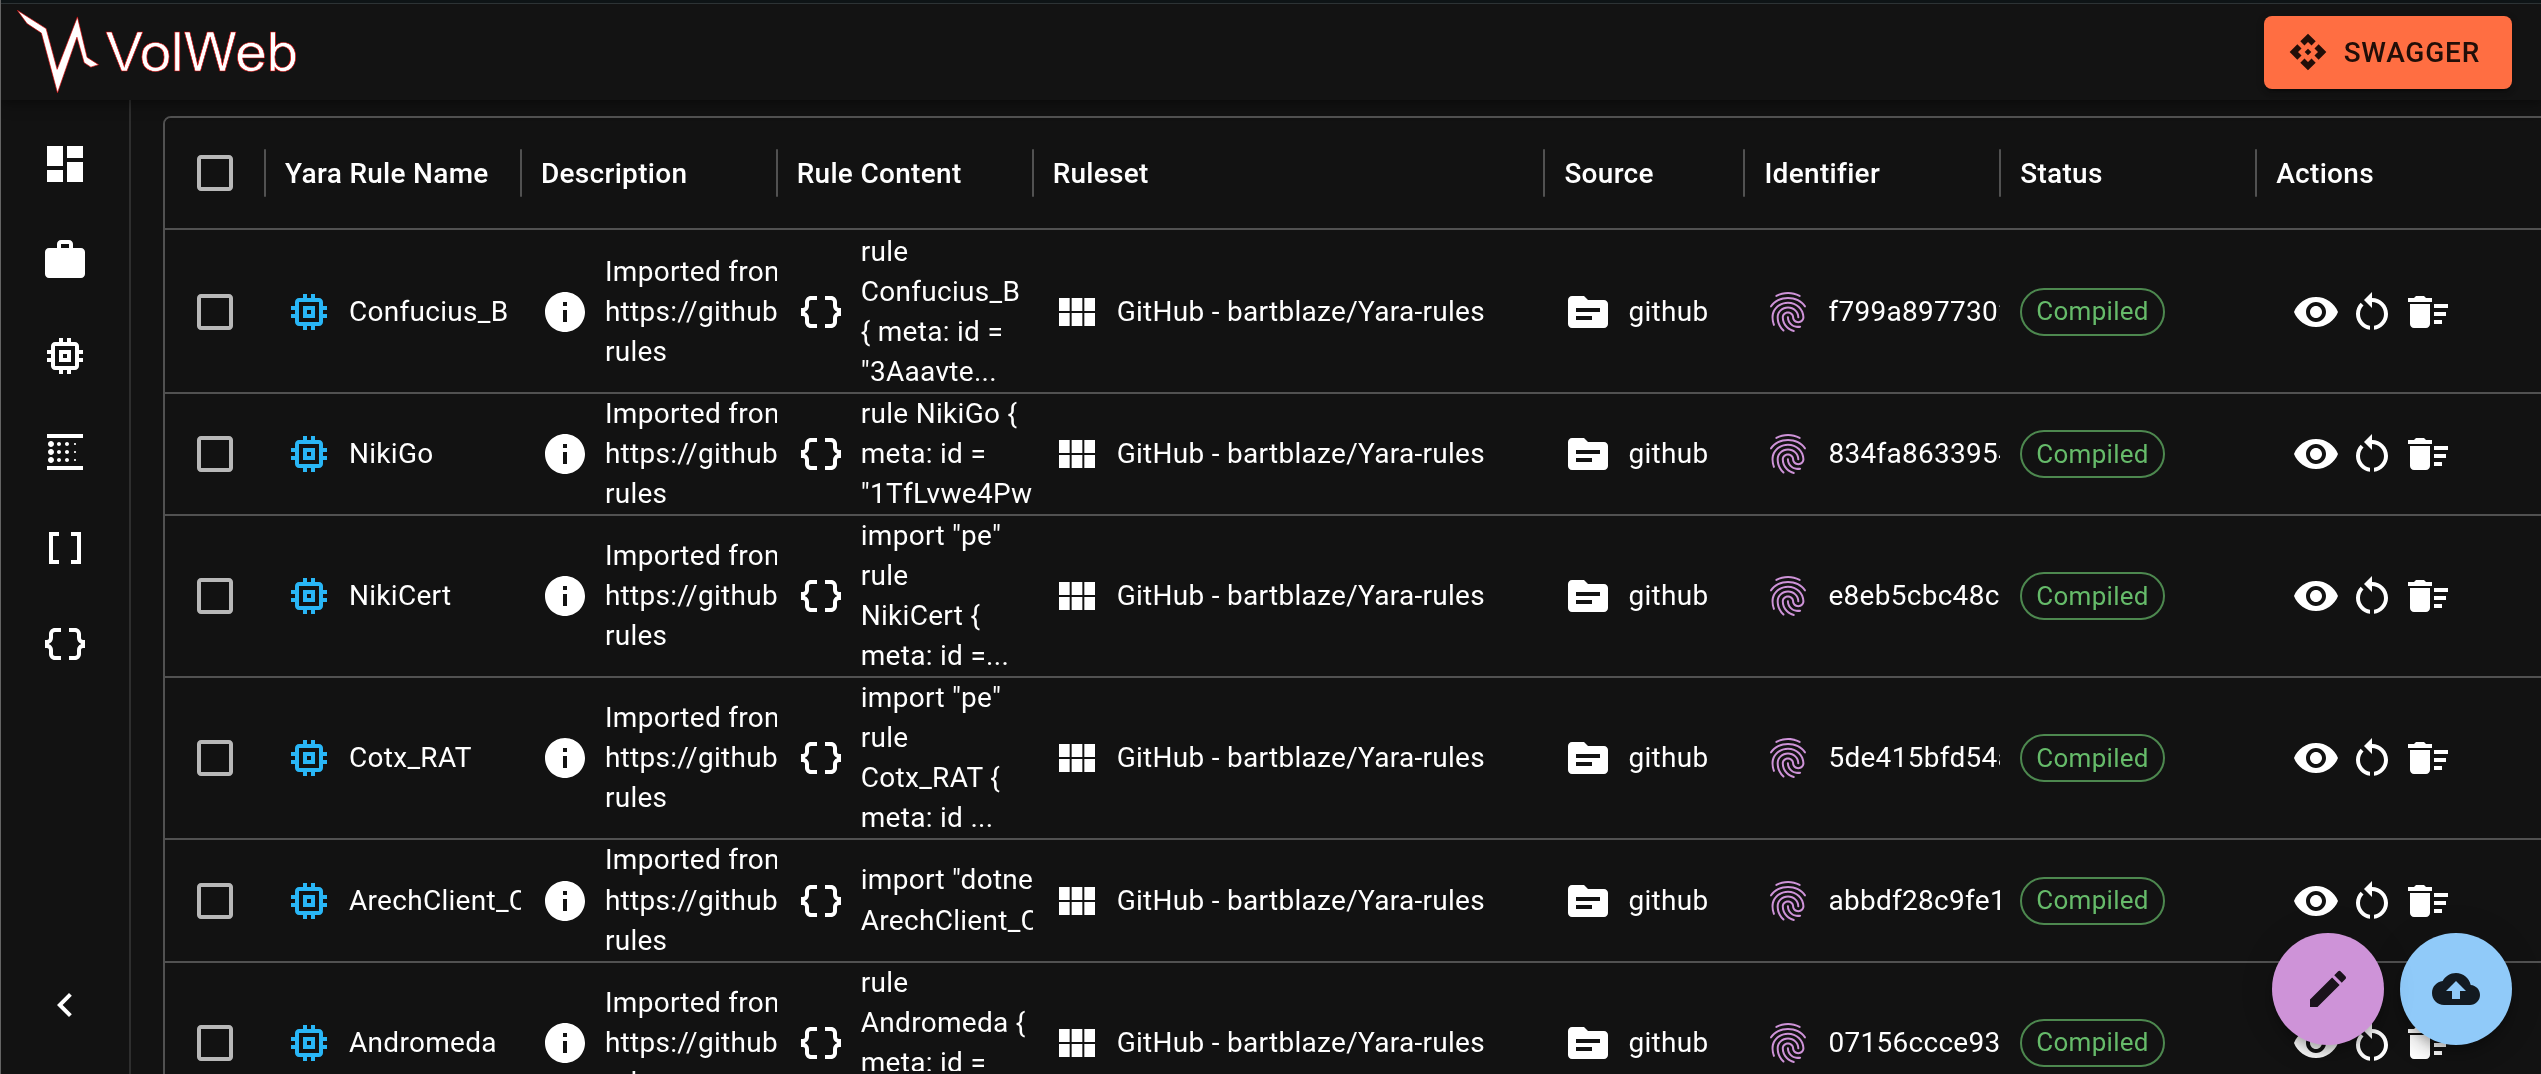
\includegraphics[width=1\linewidth]{images/volweb-esteso/volweb-rulelist.png}
\end{figure}

\subsubsection{Dialog di Import/Upload delle Regole}
Il dialog dedicato all'importazione delle regole implementa un selettore contestuale che consente all'utente di scegliere la modalità di import preferita. In particolare, è possibile caricare regole direttamente dal file system locale (upload di file) oppure effettuare l'import di intere repository ospitate su GitHub. Questa flessibilità permette di supportare sia scenari in cui le regole sono già presenti in locale, sia workflow più avanzati in cui le regole vengono versionate e mantenute tramite repository remoti, facilitando l'integrazione con pratiche di gestione collaborativa del codice.

\begin{figure}[H]
\centering
\begin{minipage}{0.45\textwidth}
\centering
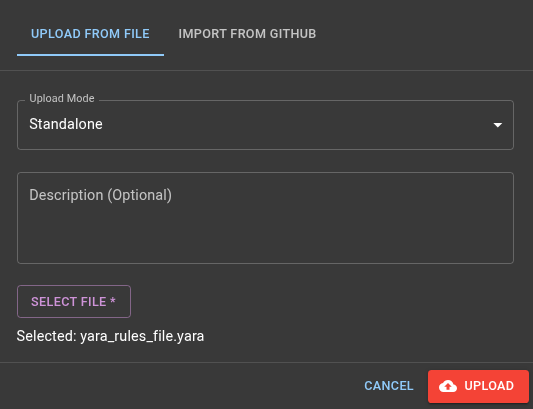
\includegraphics[width=\textwidth,height=6cm]{images/volweb-esteso/volweb-upload-dialog.png}
\end{minipage}
\hspace{0.05\textwidth}
\begin{minipage}{0.45\textwidth}
\centering
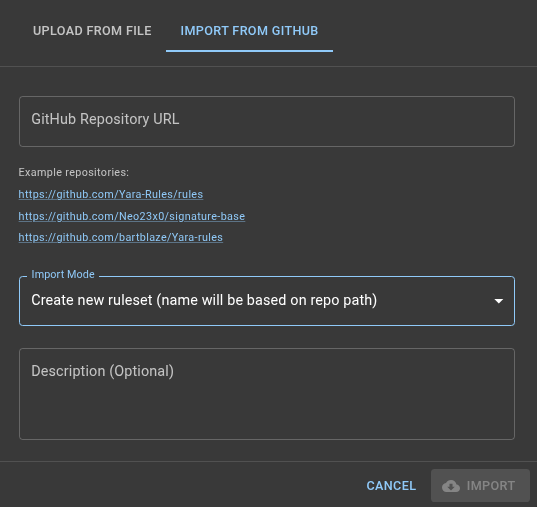
\includegraphics[width=\textwidth,height=6cm]{images/volweb-esteso/volweb-import-dialog.png}
\end{minipage}
\end{figure}

\subsubsection{Dialog per la Creazione e Modifica delle Regole}
Il dialog dedicato alla creazione e modifica delle regole integra un editor avanzato che supporta la validazione del contenuto. Questa soluzione consente agli utenti di scrivere o aggiornare le regole in modo più agevole e sicuro, evidenziando immediatamente eventuali errori sintattici o anomalie. L'adozione di un editor evoluto migliora significativamente l'esperienza d'uso, riducendo il rischio di introdurre regole non valide e favorendo un processo di definizione più rapido e affidabile.

\begin{figure}[H]
\centering
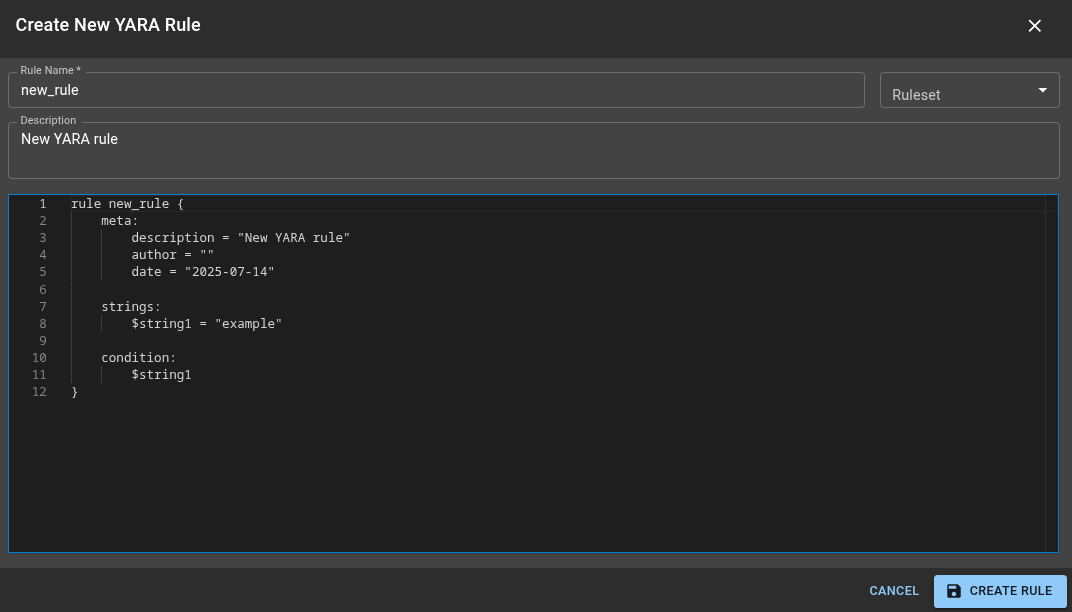
\includegraphics[width=1\linewidth]{images/volweb-esteso/volweb-creation-dialog.png}
\end{figure}

\subsubsection{Gestione dei RuleSets}

L'interfaccia per la gestione dei ruleset rappresenta un componente avanzato dell'applicazione, dedicato alla visualizzazione aggregata e alla manutenzione dei gruppi di regole YARA. Il componente \texttt{YaraRuleSetsList} mostra i ruleset in una tabella interattiva con righe espandibili, statistiche sullo stato di compilazione e pulsanti di azione rapida per validazione, clonazione, modifica e cancellazione. 

Il caricamento e l’aggiornamento dei dati avvengono tramite chiamate asincrone e notifiche via WebSocket per riflettere in tempo reale l’avanzamento delle validazioni.

\begin{figure}[H]
\centering
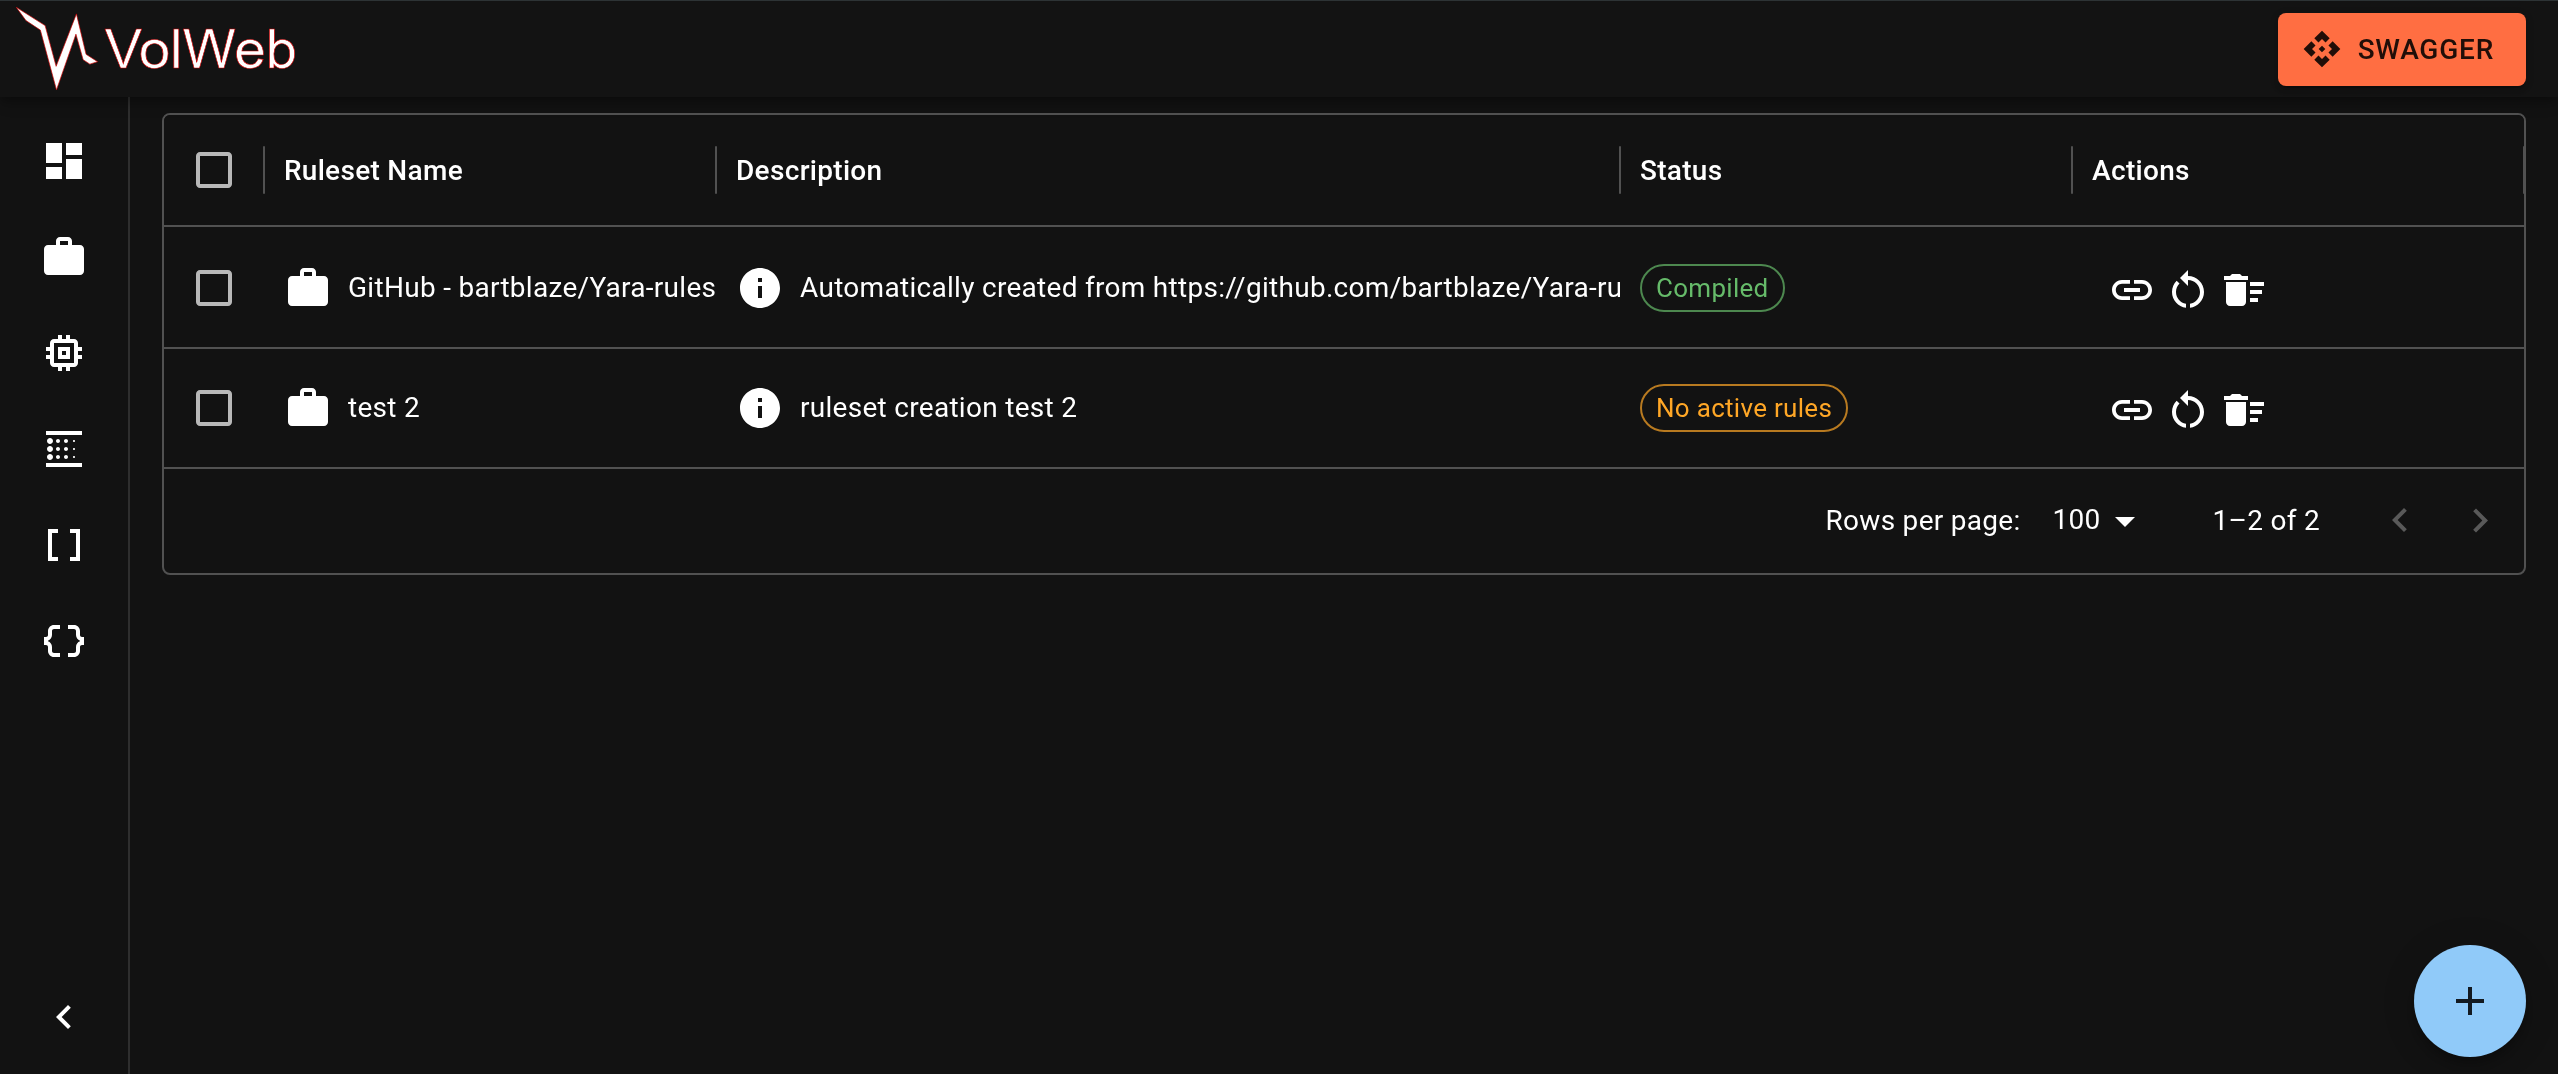
\includegraphics[width=1\linewidth]{images/volweb-esteso/volweb-rulesetlist.png}
\end{figure}


\subsubsection{Componente di Scansione}

Il componente \texttt{YaraScanDialog} costituisce l’interfaccia principale attraverso cui gli analisti configurano ed eseguono scansioni YARA sui dump di memoria. L’implementazione prevede un sistema a tab che consente di selezionare rulesets completi o regole individuali, con una validazione preventiva delle configurazioni prima dell’avvio della scansione. Il progresso viene monitorato in tempo reale tramite WebSocket, con feedback immediati sul completamento o sugli eventuali errori.

\begin{figure}[H]
\centering
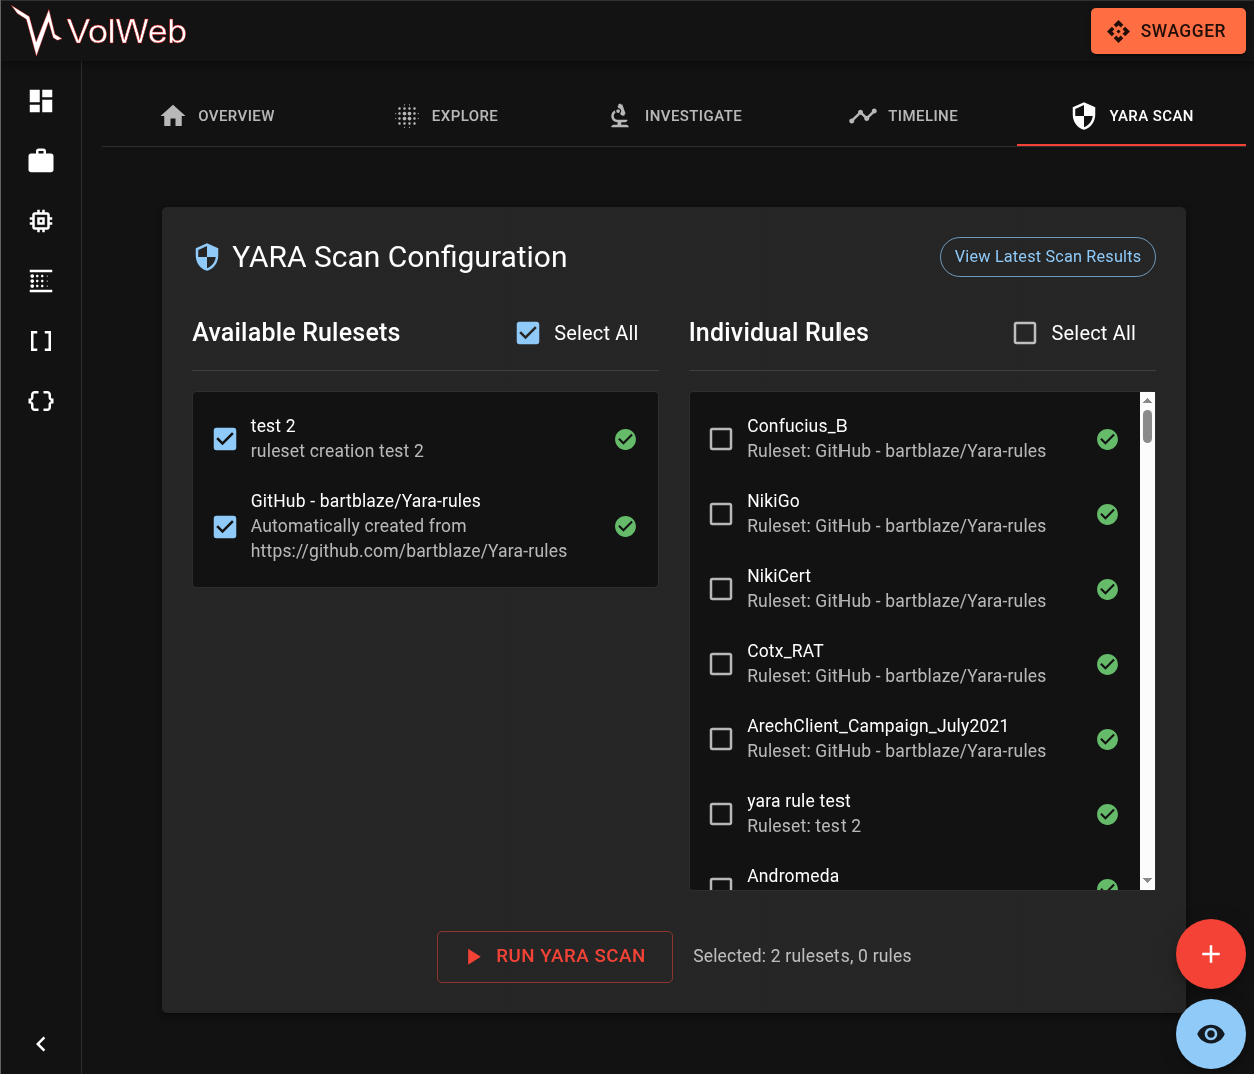
\includegraphics[width=1\linewidth]{images/volweb-esteso/volweb-scanview.png}
\end{figure}

\subsubsection{Visualizzazione dei Risultati delle Scansioni}
La visualizzazione dei risultati delle scansioni YARA rappresenta un componente critico per l'efficacia dell'analisi forense. Il componente \texttt{YaraScanResults} implementa una tabella avanzata, realizzata con il componente \texttt{DataGrid} di MUI X, che permette ordinamento, paginazione e personalizzazione delle celle. Ogni riga della tabella mostra l’offset di memoria in cui è stato rilevato il match, il nome della regola YARA che ha determinato l’individuazione, il valore effettivo che ha fatto scattare la corrispondenza e la condizione che ha portato al match

\begin{figure}[H]
\centering
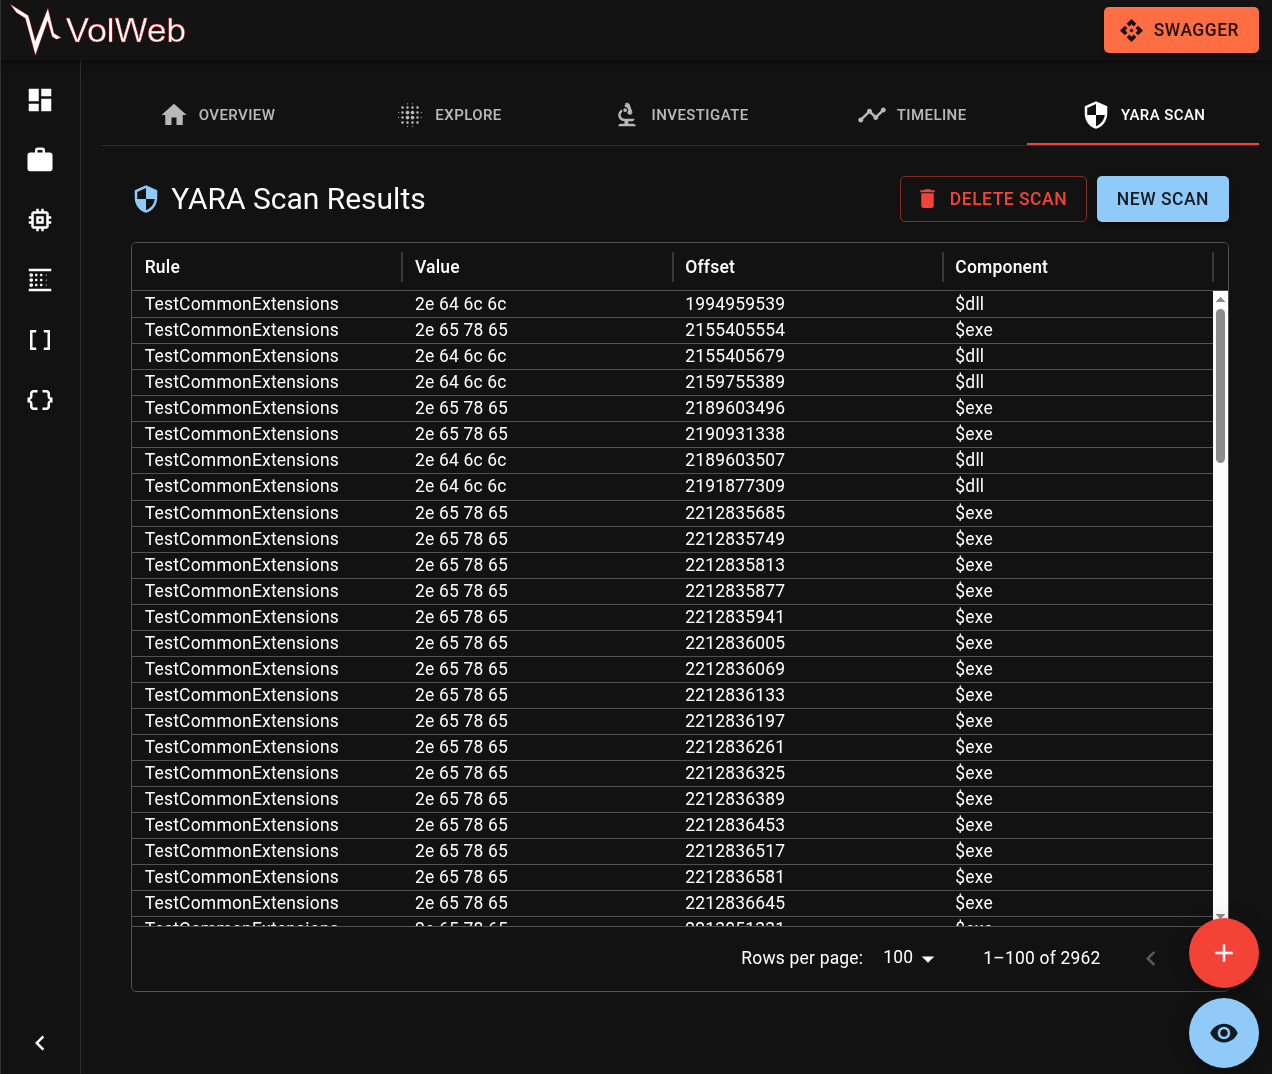
\includegraphics[width=1\linewidth]{images/volweb-esteso/volweb-scanresult.png}
\end{figure}


\section{Semplificazioni Architetturali}

Parallelamente all'integrazione YARA, sono state implementate semplificazioni architetturali significative basate sull'esperienza operativa di Locked Shields 2025.

\subsection{Rimozione del Sistema di Autenticazione}

L'eliminazione del layer di autenticazione rappresenta una decisione progettuale guidata dall'analisi del contesto operativo reale di VolWeb. Durante Locked Shields 2025, ogni blue team operava in un ambiente di rete completamente isolato, dove il controllo degli accessi era demandato all'infrastruttura e non all'applicazione. In questo scenario, la presenza di un sistema di autenticazione non solo introduceva overhead inutile, ma costituiva un vero e proprio punto debole sfruttabile dagli attaccanti.

L'esperienza sul campo ha dimostrato che le password statiche o mal protette diventavano rapidamente bersagli di attacchi di brute-force e credential stuffing, compromettendo la piattaforma e annullando i benefici di una barriera applicativa. La rimozione dell'autenticazione ha portato vantaggi immediati in termini di deployment più rapido e semplice, minore complessità operativa per gli analisti e un modello architetturale semplificato. Dal punto di vista della sicurezza, questa scelta ha permesso di eliminare un'intera classe di vulnerabilità relative a password, hash e gestione dei token, riducendo drasticamente la superficie di attacco e semplificando la configurazione senza necessità di secret keys, expiration policies o meccanismi di recovery.

\subsection{Eliminazione del Supporto Cloud Storage}

La rimozione del supporto per storage cloud (S3) deriva da considerazioni sia di sicurezza che di affidabilità operativa emerse durante Locked Shields. I dump di memoria contengono per natura dati estremamente sensibili, inclusi potenziali segreti aziendali, credenziali in chiaro, e informazioni personali. L'upload di tali dati su infrastrutture cloud introduce rischi di compliance e sicurezza che molte organizzazioni non possono accettare.

Durante l'esercitazione, è emerso inoltre che i servizi cloud rappresentavano spesso target primari per gli attacchi del red team. Affidarsi a storage cloud per evidenze forensi critiche introduce un single point of failure inaccettabile: proprio nel momento di maggior necessità durante un incident, l'infrastruttura cloud potrebbe essere compromessa, sotto attacco DDoS, o semplicemente non raggiungibile a causa di problemi di rete. 

La scelta di mantenere tutto lo storage locale garantisce che le evidenze rimangano sempre sotto il controllo diretto dell'organizzazione, accessibili anche in caso di isolamento completo della rete. Questo approccio si allinea con i principi di resilienza operativa essenziali per tool di incident response, dove la disponibilità delle evidenze non può dipendere da fattori esterni. L'eliminazione del supporto cloud ha inoltre semplificato significativamente l'architettura, rimuovendo la necessità di gestire credenziali AWS, implementare logiche di retry per operazioni di rete, o gestire la sincronizzazione tra storage locale e remoto.

Le espansioni presentate in questo capitolo trasformano VolWeb da una piattaforma di visualizzazione a uno strumento completo per l'analisi forense avanzata. L'integrazione di YARA colma il gap più critico identificato durante Locked Shields 2025, mentre le semplificazioni architetturali garantiscono che la piattaforma rimanga accessibile e resiliente anche nei contesti operativi più impegnativi. 

Tuttavia, l'implementazione di nuove funzionalità richiede una validazione rigorosa per garantirne l'efficacia in contesti operativi reali. Il prossimo capitolo presenta i risultati della sperimentazione sul campo, analizzando le performance della piattaforma estesa e la sua applicabilità in scenari di incident response concreti.